
\section{Motivation}
% Scene understanding is a prerequisite to many high level tasks for any automated intelligent machine operating in real world environments

% air sim is High-Fidelity, ours is low fide for simlicity

% a lot of time and efforts in image annotation but still inaccurate expensive. it is humanely impossible to label each pixel by hand. Specilaized softwares to do that 

% Scene classification is a significant aspect of computer vision. Convolutional neural networks (CNNs), a development of deep learning, are a well-understood tool for image classification. But training CNNs requires large-scale datasets. Transfer learning addresses this problem and produces a solution for small-scale datasets.

% A convolutional neural network (CNN) trained on ImageNet (Deng et al., 2009) significantly outperforms the best hand crafted features on the ImageNet challenge (Russakovsky et al., 2014). But more surprisingly, the same network, when used as a generic feature extractor, is also very successful at other tasks like object detection on the PASCAL VOC dataset (Everingham et al., 2010).

% Convolutional neural networks have recently obtained astonishing performance on object classifi- cation (Krizhevsky et al., 2012) and scene classification (Zhou et al., 2014). 

% Developing autonomous systems that are able to assist
% humans in everyday tasks is one of the grand challenges in
% modern computer science. One example are autonomous
% driving systems which can help decrease fatalities caused
% by traffic accidents. While a variety of novel sensors have
% been used in the past few years for tasks such as recognition,
% navigation and manipulation of objects, visual sensors are
% rarely exploited in robotics applications: Autonomous driving systems rely mostly on GPS, laser range finders, radar
% as well as very accurate maps of the environment

% Scene understanding is a prerequisite to many high level tasks for any automated intelligent machine operating in real world environments

% We also plot the confidence in the final per-pixel segmentation label predictions as the ratio of probabilities of second best label to the best label. As seen clearly in the Fig. 9, higher uncertainty occurs mostly at the object boundaries. We also tried variation ratio of the final class labels returned by using dropout for each pixel at test time[15] [23] but did not find it any more informative.

% The ability of an artificial neural network to perform a task is heavily influenced by the quality of its training set. If the training set contains examples taken from the full range of situations the network is expected to handle, the network will learn to perform the task accurately. But if important situations are missing during training, the network is likely to perform poorly when it later encounters the novel circumstances.
% In the domain of autonomous driving, we have shown that the connectionist architecture shown in Figure 1can quickly learn to steer by watching a person drive [2]. The network receives live input from a camera on the vehicle. The network is trained using back-propagation [3] to activate the output unit representing the driver’s current steering direction. After approximately four minutes of watching a person drive on a particular type of road, the network is able to take over for itself and drive at up to 55 miles per hour. Individual networks have been trained to drive in a wide variety of situations, including single and multi-lane roads with and without lane markings.

% Here we show that object detectors emerge from training CNNs to perform scene classification. As scenes are composed of objects, the CNN for scene classifica- tion automatically discovers meaningful objects detectors, representative of the learned scene categories. With object detectors emerging as a result of learning to recognize scenes, our work demonstrates that the same network can perform both scene recognition and object localization in a single forward-pass, without ever having been explicitly taught the notion of objects.

% Convolutional neural networks have recently obtained astonishing performance on object classification (Krizhevsky et al., 2012) and scene classification (Zhou et al., 2014). The ImageNet-CNN from Jia (2013) is trained on 1.3 million images from 1000 object categories of ImageNet (ILSVRC 2012) and achieves a top-1 accuracy of 57.4%. With the same network architecture, Places-CNN is trained on 2.4 million images from 205 scene categories of Places Database (Zhou et al., 2014), and achieves a top-1 accuracy of 50.0%. 

% Monitoring of winter road surface conditions during and after a snow storm is essential for most transportation agencies in Canada and other countries experiencing severe winter seasons. Information on road surface conditions can be used to assess the need for maintenance services, compare the effectiveness of different treatment methods, and evaluate the quality of the maintenance services delivered by contractors across different maintenance yards. Real-time information on road surface conditions is also valuable to the road users who can use the information to improve their travel and driving decisions such as where, when and in what mode to travel.

% discussion on pop conv nets, lenet has become hello
%  Focus on single multi-lane highway without lane markings
% wwrite about datasets like cityscape and synthia
\section{Thesis Goal}
This thesis aims at developing a machine learning model which can differentiate between lanes in a image of single or multi-lane highway. The model should be able to take image and a point coordinate as inputs and predicts the lane on which point exists.
\section{Related Work}
In this section, we will explore the research on traffic scene classification done by other computer scientists.
\subsection{Related Research: I}
\par
Convolutional Neural Network has become the conventional model for most of the Computer Vision task. In \cite{zhou2014object} the authors analyzed the inner layers of deep learning architectures. They followed a simple philosophy that objects make up a scene and if a CNN is able to do scene classification then it must be able to detect objects. They proposed that the inner layers learns the representation and is responsible for object detection. They also showed that a single Convolutional Neural Network can do both object detection/localization and scene recognition. The study also stressed on the point that although the representations learned by the layers of a deep learning network is confusing but it is substantially performs better than hand crafted features which are easy to comprehend.
\par
They discussed that there is a renowned dataset for object recognition, object localization and image classification known as ImageNet \cite{deng2009imagenet} and Places \cite{zhou2017places} for scene recognition. A convolutional neural network known as ImageNet-CNN \cite{donahue2014decaf} trained on ImageNet for object recognition achieved a good accuracy in ImageNet Challenge \cite{Russakovsky2015}. But when a network architecture same as ImageNet-CNN was trained on Places dataset for scene recognition, it astonishingly performed well and was able to do object localization through features in inner layers. Figure \ref{fig:places_cnn} shows the output of inner layers of the network trained. Hence, they concluded that a CNN can perform object localization even if it is trained to classify scenes.

\begin{figure}[H]
  \centering
  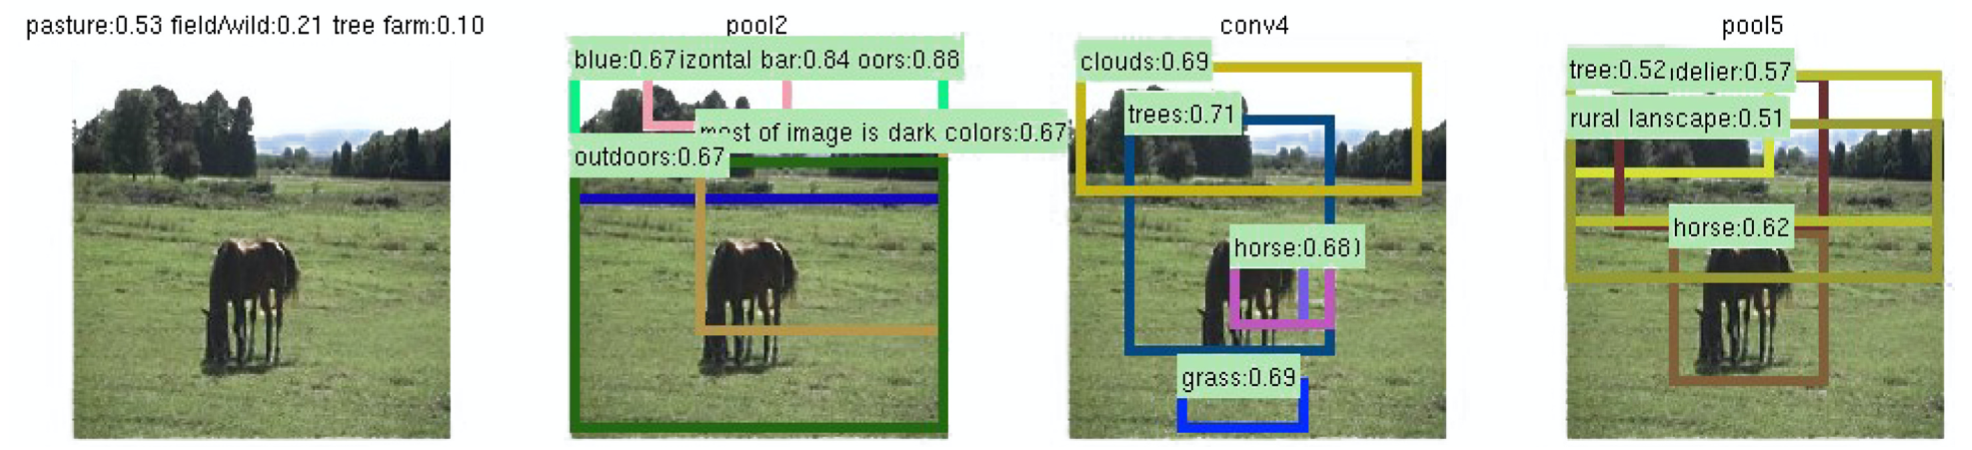
\includegraphics[scale=0.40]{images/Chapter1/places_cnn.png}
  \caption{The first images shows the recognized scene. Rest of the images show output of inner layers along with semantic tag and confidence.}
  \label{fig:places_cnn}
\end{figure}

\par
It can be helpful for our thesis because given our traffic image data we can identify the maximum number of lanes and objects like vehicles, lanes, people, traffic signs using a single CNN, without using a separate model for object detection.

\subsection{Related Research: II}
As the name \q{Training Deep Networks with Synthetic Data: Bridging the Reality Gap by Domain Randomization} suggests, this paper \cite{Training_Deep_Networks_with_Synthetic_Data}, demonstrates object detection being done a deep neural network trained on synthetic or simulated data. The author explains that not only good quality real-world labelled data in abundace is very expensive, generating large amount of photorealistic synthetic data can also become expensive. In order to cover different situations in real world, they used an approach called \q{domain randomization} \cite{domain_randomization}. Domain randomization is a process to generate complex environments in simulation with the help of different properties for example, lighting, material textures, camera viewpoints, position of objects, etc. The randomized data generated by this process can be used to train neural networks to learn important features of the object of interest. They used Faster R-CNN network with Inception ResNet V2 as the feature extractor to pre-train the network on a high-fidelity Virtual KITTI or VKITTI dataset \cite{VKITTI} and domain randomized (DR) dataset. And later fine-tune the network with real-world data. The authors proposed that the combination of using low-cost synthetic domain randomized data for pre-training and real images for fine-tuning the network is more effective than the networks trained on expensive photorealistic datasets and real data alone. They evaluated this approach by detecting cars on the KITTI dataset \cite{KITTI}. Figure \ref{dr} shows the car detection by both of the approaches.

\begin{figure}[H]
  \centering
  \includegraphics[scale=0.34]{images/Chapter1/dr.png}
  \caption{Car localization on KITTI images using Faster-RCNN trained only on synthetic data, either on the VKITTI dataset or Domain randomized dataset.}
  \label{fig:dr}
\end{figure}

\subsection{Related Research: III}
The paper \cite{omer2010automatic} analyzes the classification of road surface condition during winters using images captured from a camera mounted on a vehicle. This paper is relatable to our thesis because we are also using machine learning approach on image classification of traffic scene and we also have the same camera angle to capture image. The difference is that we are simulating the scene instead of taking images in real-world. The paper also points us to consider the changes in road conditions due to change in weather, lighting and shadows.
\par
The authors emphasize that weather conditions such as heavy snowfall can drasticly change the road conditions. Hence, a system to monitor road conditions can help in driving decisions. They used feature vectors such as RGB features and gradients to train Scalar Vector Machine (SVM) for classifying road surface conditions such as snow covered and bare.

\section{Thesis Structure}
In the following chapter, the field of Machine Learning is thoroughly examined, its history, basic concepts and related topics such as Artificial Neural Networks \cite{ann} and Convolution Neural Networks are discussed. Chapter \ref{chap:3} will comprehensively explore datasets that are being used to support this thesis. It will explain how we generated data through a computer simulation and why we needed a simulation to do that. We will show what kind of data is gathered, overview of data distribution and how we preprocessed it to be used by our machine learning model. In the next Chapter \ref{chap:4}, we will talk about the tools and technologies used for data gathering, implementation, evaluation and visualization of our solution. We will also discuss the convolution neural network we are using and how we tweaked it to fit our needs. In Chapter \ref{chap:5}, the experiments that were carried out and their results will be described. All those results will be further evaluated by some metrics and graphs. We will also show some visualiztions making our predictions easier to understand by humans by detecting patterns and outliers. In the last Chapter \ref{chap:6}, we would review all the research we have done in order to explain what we have learnt from the findings and whether or not this study is successful in solving the mentioned problem. Finally, there will be discussion of future work, followed by all tasks which were planned, but not completed because of time limits.